\begin{tikzpicture}[font=\scriptsize, >=Latex]
\node[draw=mavebline, rounded corners=2pt, very thick, fill=mavebblue,
      minimum width=0.28\textwidth, minimum height=2.7cm, align=center] (s0) at (0,0) {};
\node[draw=mavebline, rounded corners=2pt, very thick, fill=mavebblue,
      minimum width=0.28\textwidth, minimum height=2.7cm, align=center] (s1) at (5.0,0) {};
\node[draw=mavebline, rounded corners=2pt, very thick, fill=mavebamber,
      minimum width=0.28\textwidth, minimum height=2.7cm, align=center] (s2) at (10.0,0) {};
\node[anchor=north west,font=\small\bfseries] at ($(s0.north west)+(0.12,-0.12)$) {1  Initial Gaussian state};
\node[anchor=north west,font=\small\bfseries] at ($(s1.north west)+(0.12,-0.12)$) {2  Intended edit / movement};
\node[anchor=north west,font=\small\bfseries] at ($(s2.north west)+(0.12,-0.12)$) {3  Certified support formation};
\foreach \x/\y/\r/\c in {-0.65/-0.2/0.28/gray!55,-0.25/0.25/0.34/gray!70,0.1/-0.18/0.31/gray!60,
                          0.46/0.24/0.29/gray!75,0.74/-0.12/0.25/gray!50,-0.05/0.55/0.24/gray!50}
  \fill[\c,opacity=.78] ($(s0.center)+(\x,\y)$) circle (\r);
\foreach \x/\y/\r/\c in {-0.65/-0.2/0.28/gray!55,-0.25/0.25/0.34/gray!70,0.1/-0.18/0.31/gray!60,
                          0.46/0.24/0.29/gray!75,0.74/-0.12/0.25/gray!50,-0.05/0.55/0.24/gray!50}
  \fill[\c,opacity=.78] ($(s1.center)+(\x-0.15,\y)$) circle (\r);
\fill[blue!65,opacity=.88] ($(s1.center)+(0.95,0.55)$) circle (.28);
\draw[->,very thick,draw=mavebline] ($(s1.center)+(0.35,0.42)$) -- ($(s1.center)+(0.82,0.52)$);
\foreach \x/\y/\r/\c in {-0.65/-0.2/0.28/gray!55,-0.25/0.25/0.34/gray!70,0.1/-0.18/0.31/gray!60,
                          0.46/0.24/0.29/gray!75,0.74/-0.12/0.25/gray!50,-0.05/0.55/0.24/gray!50}
  \fill[\c,opacity=.65] ($(s2.center)+(\x-0.1,\y)$) circle (\r);
\fill[yellow!70,opacity=.95] ($(s2.center)+(0.45,0.05)$) circle (.42);
\fill[yellow!70,opacity=.95] ($(s2.center)+(0.78,0.35)$) circle (.32);
\fill[blue!65,opacity=.95] ($(s2.center)+(0.95,0.55)$) circle (.25);
\draw[yellow!60!black,very thick,dashed] ($(s2.center)+(0.58,0.18)$) circle (.78);
\node[anchor=west] at ($(s2.center)+(1.25,0.55)$) {edited Gaussian};
\node[anchor=west] at ($(s2.center)+(1.25,0.12)$) {certified support};
\draw[->,very thick,draw=mavebline] (s0.east) -- (s1.west);
\draw[->,very thick,draw=mavebline] (s1.east) -- (s2.west);
\node[draw=mavebline,rounded corners=2pt,very thick,fill=white,
      minimum width=0.94\textwidth,minimum height=3.0cm] (pipeline) at (5,-3.6) {};
\node[anchor=north west,font=\small\bfseries] at ($(pipeline.north west)+(0.12,-0.12)$)
      {State transition pipeline};
\node[anchor=north west,text=mavebline] at ($(pipeline.north west)+(2.8,-0.14)$)
      {edit $\rightarrow$ support $\rightarrow$ repair or \FULL{} $\rightarrow$ oracle};
\node[inner sep=0pt] at ($(pipeline.center)+(0,-0.20)$)
      {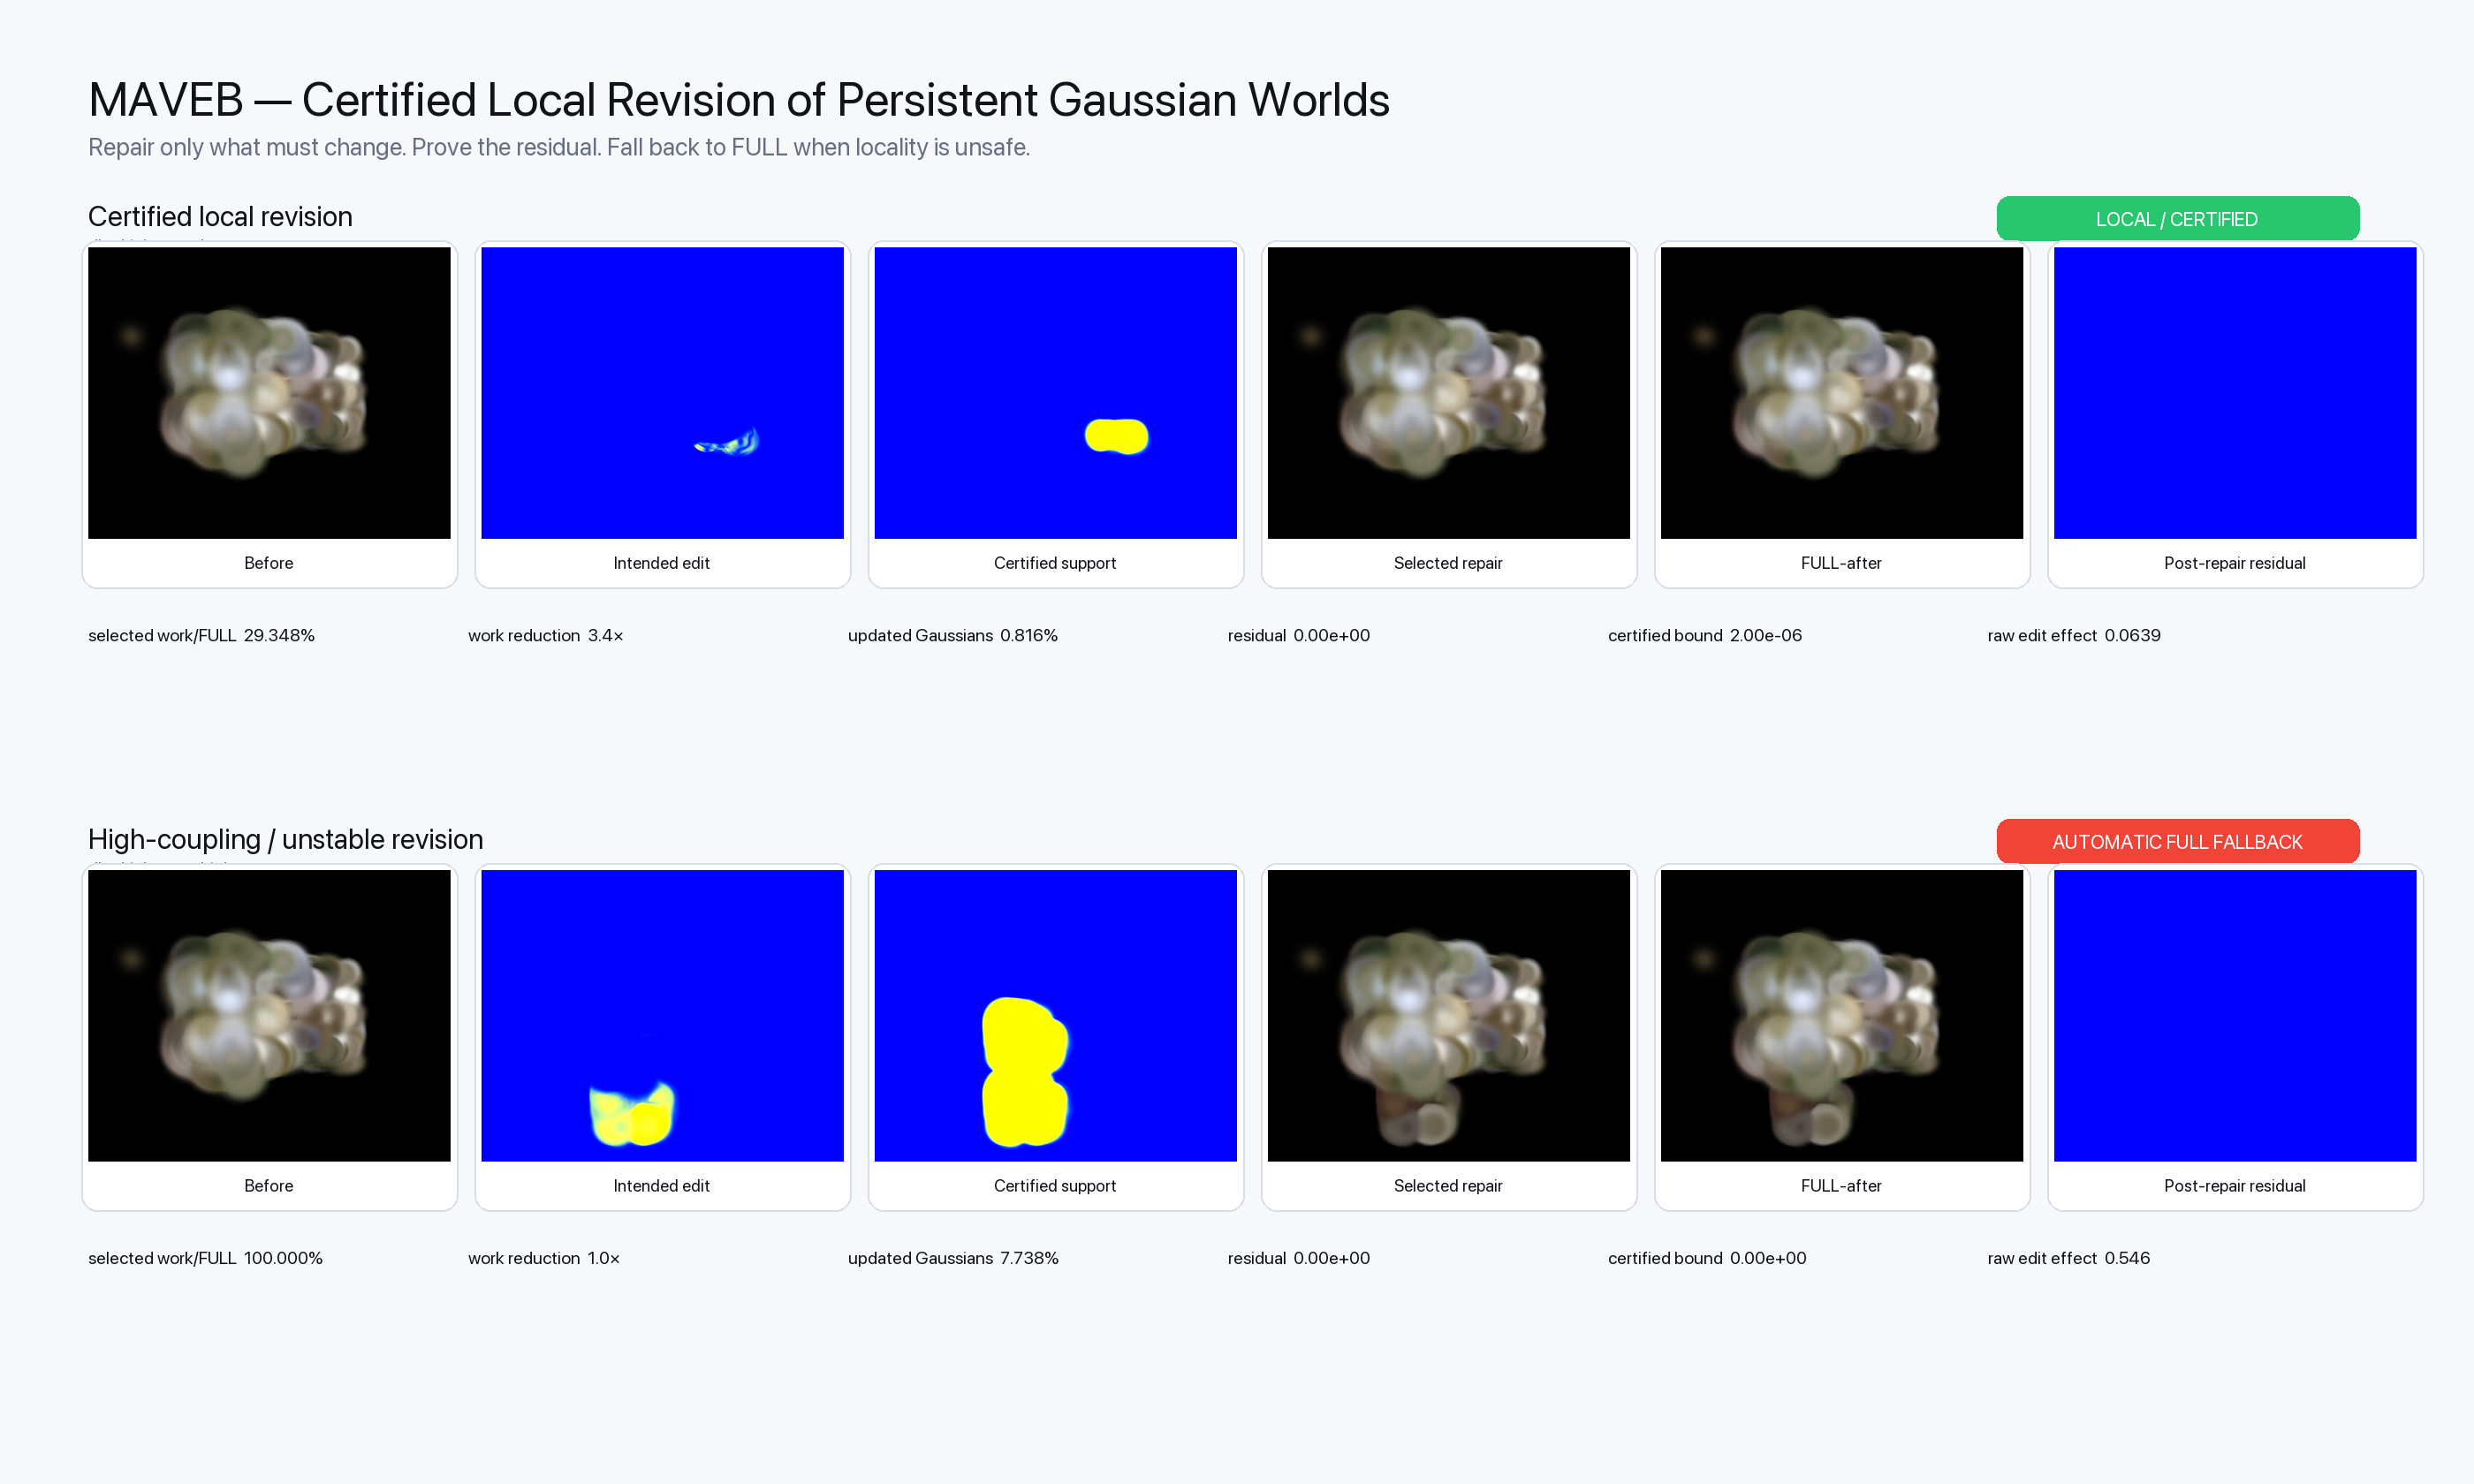
\includegraphics[width=0.86\textwidth]{../research/results/visualizations/public/F0_hero.png}};
\node[draw=green!55!black,rounded corners=2pt,very thick,fill=mavebgreen,
      minimum width=0.45\textwidth,minimum height=2.25cm,align=left,text width=0.41\textwidth] (ok) at (2.5,-7.1)
      {\textbf{\large A \quad Certified local repair}\\[4pt]
       Repair only the selected support. The remainder of the scene stays unchanged.\\[3pt]
       \textbf{Accept when:} certificate is feasible, measured work is below \FULL{}, and oracle replay respects the bound.};
\node[draw=red!65!black,rounded corners=2pt,very thick,fill=mavebrose,
      minimum width=0.45\textwidth,minimum height=2.25cm,align=left,text width=0.41\textwidth] (bad) at (7.5,-7.1)
      {\textbf{\large B \quad Automatic \FULL{} fallback}\\[4pt]
       Rebuild when coupling is too broad, a bound fails, assumptions are unsupported, or local work crosses the full baseline.\\[3pt]
       \textbf{Purpose:} preserve the stated output contract instead of forcing locality.};
\coordinate (decision) at (5,-5.55);
\draw[->,very thick,draw=green!55!black] (decision) -- (2.5,-5.55) -- (ok.north);
\draw[->,very thick,draw=red!65!black] (decision) -- (7.5,-5.55) -- (bad.north);
\node[fill=white,inner sep=2pt] at (5,-5.55) {\textbf{check certification and work criteria}};
\end{tikzpicture}
